\documentclass{beamer}

%% Configuración de la presentación
\mode<presentation> {

  \usetheme{Warsaw}

  
  \usecolortheme{beaver}
 
}

%% Fuentes de tamaño arbitrario
\usepackage{lmodern}
\usepackage{amsfonts}
\usepackage{dsfont}


%% Gráficos
\usepackage{graphicx} % Allows including images
\usepackage{booktabs} % Allows the use of \toprule, \midrule and \bottomrule in tables

%%% Castellano.
% noquoting: Permite uso de comillas no españolas.
% lcroman: Permite la enumeración con numerales romanos en minúscula.
% fontenc: Usa la fuente completa para que pueda copiarse correctamente del pdf.
\usepackage[english,spanish,es-noquoting,es-lcroman]{babel}
\usepackage[utf8]{inputenc}
\usepackage[T1]{fontenc}
\selectlanguage{spanish}

\usepackage{tikz}
\usepackage{tikz-cd}
\usepackage{tikz-3dplot}

\usepackage{verbatim}
\usetikzlibrary{arrows,shapes}
\usepackage{amsthm}
\usepackage{accents}
\usepackage{amsmath,amssymb,lmodern}
\usepackage{fontawesome}
\usepackage{setspace}
\usepackage{subfig}

% Definitions
\theoremstyle{plain}
\newtheorem{thm}{Teorema}
\theoremstyle{definition}
\newtheorem{defn}[thm]{Definición}
\theoremstyle{plain}
\newtheorem{prop}[thm]{}
\theoremstyle{definition}
\theoremstyle{remark}
\newtheorem{rem}[thm]{Nota}
\theoremstyle{definition}
\newtheorem{lem}[thm]{Lema}
\newtheorem{cor}[thm]{Corolario}
\newtheorem{ejemplo}[thm]{Ejemplo}
\newtheorem{ejemplos}[thm]{Ejemplos}
% Counter

\newcounter{saveenumi}
\newcommand{\seti}{\setcounter{saveenumi}{\value{enumi}}}
\newcommand{\conti}{\setcounter{enumi}{\value{saveenumi}}}

% Sections
\AtBeginSection{\frame{\sectionpage}}
\newtranslation[to=spanish]{Section}{Sección}

%comandos para agilizar la escritura de simbolos frecuentes
\newcommand{\sphere}{\mathds{S}^{d-1}}
\newcommand{\esfera}{\mathds{S}^{2}}
\newcommand{\orto}{\mathbb{O}^d}
\newcommand{\R}{\mathds{R}^d}
\newcommand{\spharm}{\mathds{Y}^d_n}
\newcommand{\sphint}{\int_{\sphere}}

\defbeamertemplate{section page}{mine}[1][]{%
  \begin{centering}
    {\usebeamerfont{section name}\usebeamercolor[fg]{section name}#1}
    \vskip1em\par
    \begin{beamercolorbox}[sep=12pt,center]{part title}
      \usebeamerfont{section title}\insertsection\par
    \end{beamercolorbox}
  \end{centering}
}

%----------------------------------------------------------------------------------------
%	TÍTULO
%----------------------------------------------------------------------------------------

\title[]{Análisis y monitorización de aplicaciones a través de plugins con Naemon} % The short title appears at the bottom of every slide, the full title is only on the title page

\author{Sofía Fernández Moreno} % Your name
\institute[UGR] % Your institution as it will appear on the bottom of every slide, may be shorthand to save space
{
  Universidad de Granada \\ % Your institution for the title page
  % Your email address
}
\date{Septiembre de 2019} % Date, can be changed to a custom date

% logo of my university
\titlegraphic{
	
\includegraphics[width=2cm]{imagenes/logo_ugr.jpg}
	
\includegraphics[width=2cm]{imagenes/etsiit_logo.png}
}


\begin{document}
% Spanish
\selectlanguage{spanish}
% Para tikz
\pgfdeclarelayer{background}\theoremstyle{definition}
\pgfsetlayers{background,main}
% Secciones
\setbeamertemplate{section page}[mine]

%% Diapositiva de título.
\frame{\titlepage}

%% Diapositiva de contenidos.
% Throughout your presentation, if you choose to use \section{} and \subsection{} commands,
% these will automatically be printed on this slide as an overview of your presentation
%\begin{frame}
%  \frametitle{Contenidos} % Table of contents slide, comment this block out to remove it
%  \tableofcontents
%\end{frame}


%----------------------------------------------------------------------------------------
%	PRESENTACIÓN
%----------------------------------------------------------------------------------------

%------------------------------------------------
\section{Estado del arte} % Sections can be created in order to organize your presentation into discrete blocks, all sections and subsections are automatically printed in the table of contents as an overview of the talk
%------------------------------------------------

\subsection{¿Qué es la monitorización?}
\begin{frame}
	\frametitle{¿Qué es la monitorización?}
	\begin{defn}
		La \textbf{monitorización} es aquella en la que se toman las medidas preventivas y
		consecuentes con la información que se obtienen de todos los dispositivos
		que se encuentran conectados a una red, para evitar posibles eventos que
		hacen que se interrumpan el correcto funcionamiento de alguno de ellos
	\end{defn}
Dentro de este concepto es importanteaplicar el uso del protocolo \textbf{SNMP} (Simple Network
Management Protocol).
\begin{prop}
	\textbf{SNMP} permite el intercambio de información amplia entre los diferentes dispositivos de red mediante consultas de forma remota (polling) y mediante mensajes basándose en eventos (traps).
\end{prop}

	
\end{frame}

\subsection{Comparativa herramientas de monitorización}
\begin{frame}
	\frametitle{Comparativa herramientas de monitorización}
	\centering
	
\includegraphics[scale=0.5]{imagenes/comparativaMonitorizacion.png}
\end{frame}

\subsection{Naemon}
\begin{frame}
	\frametitle{Funcionamiento}
	\begin{itemize}
		\item Basado en Nagios 4.0.2, funcionando de la misma forma mediante representación de la monitorización a través de host y servicios concretos.
		\item Monitorización de servicios de red
		\item Monitorización de recursos de un host
		\item Diseño de plugins o complementos
	\end{itemize}
\begin{block}
	
	Podemos encontrar cuatro estados en los chequeos: \textbf{OK,
	WARNING, CRITICAL y UNKNOWN}
\end{block}
	
\end{frame}
\begin{frame}
	\frametitle{Archivo de configuración principal}
	\centering
	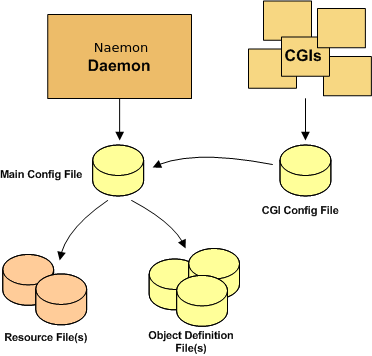
\includegraphics[scale=0.5]{imagenes/main_configuring.png}
		
\end{frame}

\begin{frame}
	\frametitle{Tipos de objetos}
	\begin{prop}
		La \textbf{configuración} de los distintos equipos y servicios a monitorizar se puede realizar a través de la carpeta \textbf{/etc/naemon/conf.d}
	\end{prop}
Podemos encontrar como objetos de definición:
\begin{itemize}
	\item Hosts
	\item Servicios
	\item Comandos
	\item Contactos
	\item Time Periods
\end{itemize}
	
\end{frame}

\begin{frame}
	\frametitle{Interfaz GUI: Thruk}
	\centering
	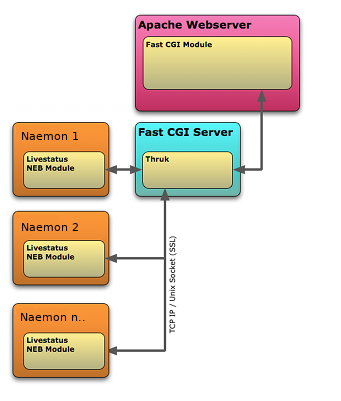
\includegraphics[scale=0.5]{imagenes/arquitecturaThruk.png}
	
\end{frame}
\begin{frame}
	\frametitle{Uso de plugins}
	\begin{block}
		
		Los \textbf{plugins} actúan como una capa de abstracción entre la lógica de supervisión presente en el demonio de Naemon y los servicios y hosts reales que se están supervisando.
	\end{block}
	\centering
	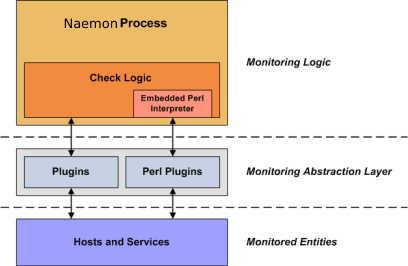
\includegraphics[scale=0.3]{imagenes/plugins.png}
	
	\begin{prop}
		El inconveniente de usar plugins en Naemon es que éste no tiene reflejo de qué es lo que está monitorizando, simplemente rastrea los cambios en el estado de esos recursos.
	\end{prop}
	
\end{frame}

\section{Realización del despliegue de Naemon} % Sections can be created in order to organize your presentation into discrete blocks, all sections and subsections are automatically printed in the table of contents as an overview of the talk
%------------------------------------------------


\subsection{Entorno de desarrollo}
\begin{frame}
	\frametitle{Uso de contenedores}
	\centering
	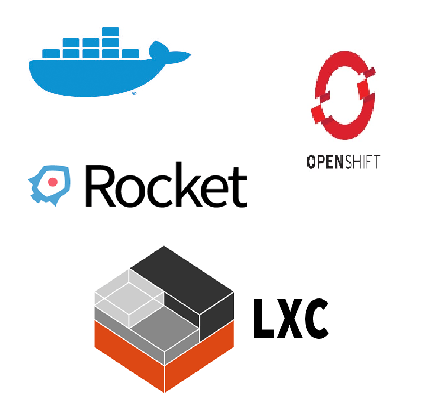
\includegraphics[scale=0.4]{imagenes/comparativaContenedores.png}
	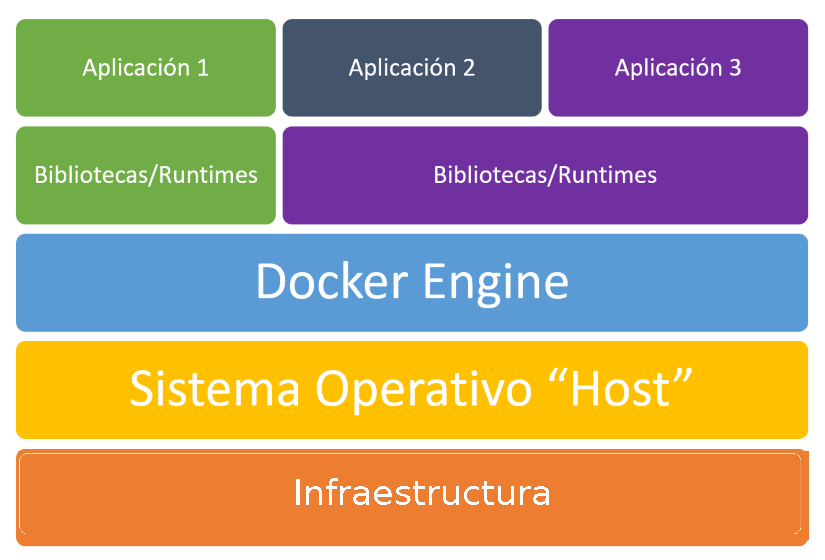
\includegraphics[scale=0.3]{imagenes/contenedores.png}
	
\end{frame}
\subsection{Desarrollo de despliegue}
\begin{frame}
	\frametitle{Creación de archivo Dockerfile}
	\begin{prop}
		
		Para poder realizar el despliegue tendremos que crear el fichero \textbf{Dockerfile}. Con este fichero construiremos la imagen de Naemon de forma automática, leyendo las instrucciones que le indiquemos.
	\end{prop}
	\centering
	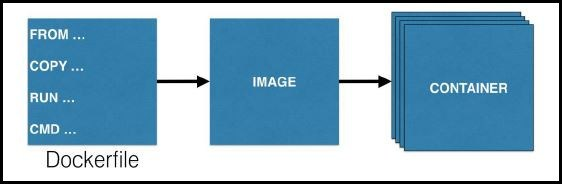
\includegraphics[scale=0.4]{imagenes/dockerfile-image.png}
	
\end{frame}


\begin{frame}
	\centering
	\includegraphics[scale=0.08]{imagenes/dockerfile-Naemon.png}
\end{frame}
\begin{frame}
		\frametitle{Archivo de ejecución ENTRYPOINT}
	\centering
	\includegraphics[scale=0.2]{imagenes/runbash1.png}
	\includegraphics[scale=0.2]{imagenes/runbash2.png}
\end{frame}

\begin{frame}
	\frametitle{Orquestación estática de aplicaciones}
	\begin{defn}
		La \textbf{orquestación estática} es aquella que el sistema requiere una configuración más
		manual de los recursos y no permite el escalado de forma muy eficiente.
	\end{defn}
\end{frame}
\begin{frame}
	\frametitle{Docker-Compose}
	Permite la orquestación estática orientada a un funcionamiento más centrado en un solo servidor, esta nos permite a través de un fichero YML,	la definición y ejecución de aplicaciones Docker en múltiples contenedores.
	\centering
	\includegraphics[scale=0.1]{imagenes/docker-compose1.png}
\end{frame}
\section{Pruebas de carga} 
	\begin{defn}
	La \textbf{prueba de carga} se trata de una prueba que generalmente observa el comportamiento de una aplicación bajo una serie de peticiones.
\end{defn}
	\begin{defn}
	La prueba de estrés se utiliza como su propio nombre dice estresar la aplicación, es decir, que se encuentre en un estado forzado.
\end{defn}
	\begin{defn}
	La prueba de estabilidad se trata de una prueba que generalmente observa el comportamiento de una aplicación bajo una serie de peticiones.
\end{defn}
	\begin{defn}
	La prueba de carga se trata de una prueba que generalmente observa el comportamiento de una aplicación bajo una serie de peticiones.
\end{defn}

\subsection{Pruebas de rendimiento}
\begin{frame}
	\frametitle{Tipos de pruebas}
	
\end{frame}
\begin{frame}
	\frametitle{Elección a realizar}
	
\end{frame}

\subsection{Comparativa de herramientas}
\begin{frame}
	\frametitle{Comparativa de herramientas}
	
\end{frame}

\subsection{Locust}
\begin{frame}
	\frametitle{Funcionamiento de Locust}
	
\end{frame}
\begin{frame}
	\frametitle{Locustfile}
\end{frame}
\section{Pruebas de carga en un sistema} % Sections can be created in order to organize your presentation into discrete blocks, all sections and subsections are automatically printed in the table of contents as an overview of the talk
%------------------------------------------------


\subsection{Locust en Docker-Compose}
\begin{frame}
	\frametitle{Enlazado de Locust}
	
\end{frame}
\begin{frame}
	\frametitle{Resultados}
	\end{frame}
\subsection{Naemon en Docker-Compose}
\begin{frame}
	\frametitle{Creación de host y servicios}
	
\end{frame}
\begin{frame}
	\frametitle{Creación de plugin como ejemplo}
	
\end{frame}
\begin{frame}
	\frametitle{Resultados}
	\end{frame}


\section{Modelado de las pruebas} % Sections can be created in order to organize your presentation into discrete blocks, all sections and subsections are automatically printed in the table of contents as an overview of the talk
%------------------------------------------------
\subsection{Carga de trabajo}
\begin{frame}
	\frametitle{¿Qué es la carga de trabajo?}
	\begin{defn}
		La \textbf{carga de trabajo} es el conjunto de todas las peticiones que el sistema recibe de su entorno
		durante un periodo de tiempo dado.
	\end{defn}
El análisis de la carga es un papel fundamental en cualquier
estudio en los que hay que determinar \textbf{índices de rendimiento}, estos se
encuentran directamente relacionados con la carga y no se pueden expresar
de forma independiente a ésta. Además el índice de rendimiento siempre debe
ir determinado de la información de la carga bajo la que fue determinado.
	
\end{frame}
\subsection{PNP4Nagios}

\begin{frame}
	\frametitle{PNP4Nagios en Dockerfile}
\end{frame}
\begin{frame}
	\frametitle{Captura de resultados}
	Añadir demo.mp4
\end{frame}


\section{Conclusiones y futuros trabajos}
\subsection{Conclusiones}
\begin{frame}
	\frametitle{Conclusiones}
	En cuanto a los resultados obtenidos en dicho análisis se aprecia
	como el sistema responde de forma positiva durante los treinta minutos de
	comprobación, ya que no pierde paquetes a la hora de realizar el PING,
	aplicando tiempos RTA bastante reducidos, además a la hora de mandar
	peticiones HTTP, éste responde de forma favorable puesto que los tiempos
	de respuesta son lo suficientemente pequeños para que no haya problemas
	de pérdida de conexión, además el tamaño de los paquetes generados son
	siempre los mismos por lo que no tendremos ninguna desfragmentación generada.
	
\end{frame}
\subsection{Trabajos futuros}
\begin{frame}
	\frametitle{Trabajos futuros}
En cuanto a los trabajos futuros a partir del actual, el principal
sería la realización de forma automatizada del despliegue pudiendo apoyar-
nos de la herramienta \textbf{Ansible}. Otra idea futura sería la adaptación de la
pila \textbf{ELK(Elasticsearch, Logstash y Kibana)} de \textbf{Elastic} para recoger todos
los registros generados durante la monitorización, haciendo que la búsqueda, análisis y visualización de los datos aparezcan con mayor facilidad en
los dashboard, además de poder manejarse gran cantidad de datos de forma
eficiente.	
\end{frame}
\subsection{}
\begin{frame}{}{}
	\Huge{\centerline{Gracias por su atención}}
	\centerline{\Huge{\raisebox{-.25\height}\faGithub}~\large{\href{https://github.com/sofiafernandezmoreno/TFG}{\alert{sofiafernandezmoreno/TFG}}}}

\end{frame}
\end{document}